After finishing the variance analysis 
writing reports on my work 
for P. Jacquet and my supervisor, I started
working on a new task.
A the heart of it remains the proof of the central limit theorem for 
LZ'78 on Markov sources - and the results that fall from it such
as the precise analysis of the convergence rate to entropy.
In the yet unpublished~\cite{jacquet_towards_nodate}, Philippe 
and Wojciech have been working on a new path to proving it.
The difficulty of Markov sources is the dependency between
phrases, which makes it hard to analyze the behavior of 
$M_n$ - the number of such phrases. Their idea is to 
first do the analysis of a simpler variable which is the 
tail symbols count that we will introduce now. We do so 
in a new simulation model : the \emph{\bfseries Markov Independent Model}.

\section{Markov Independent Model}

Let $M$ be a Markov source and $n$ an integer.
The \emph{\bfseries Markov Independent Model} (MI) considers $n$ sequences 
generated by $M$. The choice of the starting symbol of each sequence
is a parameter of the model. For example, all the sequences
might start with the same letter of the alphabet $c \in \mathcal{A}$.
Or the first symbol could be initialized using the stationary distribution
of the Markov chain related to $M$.

\noindent
This is an example for $n = 4$. These are the sequences :

\[
\begin{array}{cl}
  X(1) &= 00000\dots \\
  X(2) &= 1010101\dots \\
  X(3) &= 1001101\dots \\
  X(4) &= 001100111\dots
\end{array}
\]

\setlength{\parindent}{0pt}
These sequences are used to build a digital search tree
by considering the shortest prefix of each sequence 
that has not appeared yet in the previously considered sequences.
On our example, it yields the parsed word :
  \centers{$()(0)(1)(10)(00)$}
which can be read as the DST :
\centers{
  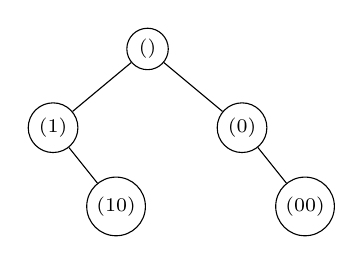
\begin{tikzpicture}[
      level 1/.style={level distance=10mm,sibling distance=24mm},
      level 2/.style={level distance=10mm,sibling distance=16mm},
      level 3/.style={level distance=10mm,sibling distance=16mm},
      font=\scriptsize,inner sep=2pt,every node/.style={draw,circle,minimum size=3ex}]
    ]
    \node {()}
      child {node {(1)}
          child[missing]
          child {node {(10)}}
      }
      child {node {(0)}
          child[missing]
          child {node {(00)}}
      }
          ;
  \end{tikzpicture}
  }

\section{Tail symbols}

\subsection{Definition}

Each of the $n$ sequences possesses a tail
symbol. For each sequence, its \emph{\bfseries tail symbol} is the character that
immediately follows the prefix phrase inserted into the DST.
Therefore the tail symbol is a specific character of this sequence.
If we only have the DST containing the prefix phrases, we cannot
recover the tail symbols.

Visually, with the \textcolor{red}{prefix phrases} in red and the 
\textcolor{green}{tail symbol} in green :

\begin{egalites}
  & X(1) 
    & {\color{red}{0}} {\color{green}{0}} 00000\dots \\
  &X(2) 
    & {\color{red}{1}} {\color{green}{0}}10101\dots \\
  & X(3) 
    & {\color{red}{10}} {\color{green}{0}} 1101 \dots \\
  & X(4) 
    & {\color{red}{00}} {\color{green}{1}} 100111\dots
\end{egalites}

\begin{df}
  Let $c$ be a character from our alphabet $\{ a, b \}$.
  In the case when \emph{all the sequences start with a $c$}, we 
  define \emph{\bfseries $T_n^{\,c}$} the \emph{\bfseries number of times $a$ is a tail symbol in 
  the experiment}.
\end{df}

\begin{rmk}
  \label{rmk:alphaet}
  This is a general definition: for example, in our simulations,
  the alphabet is $\{0, 1\}$ and we only study $T_n^{\,0}$ while
  having all our sequences start with a 0 (initialization step).
\end{rmk}

\subsection{Recurrence relation}

For $n \geq 0$, we have :
    \[ \boxed{ T_{n+1}^{\,c} = \delta_a + 
                            {{\tilde T}_{N_a}}^a
                            + {{\tilde T}_{N_b}}^b } \]

where :
\begin{itemize}
  \item $\delta_a = 
            \begin{cases} 
                1 & \text{if $a$ is the tail symbol of the
                          first sequence}\\
                0 & \text{else} 
              \end{cases}$

  \item $N_a$ is the 
random variable giving \emph{the size of the left subtree 
which contains phrases whose second letter is $a$}

  \item ${{\tilde T}_{N_a}}^a$ is the number of 
times $a$ is a tail symbol for the sequences that were 
used to  build the subtree with phrases having $a$ as second
symbol.

  \item $T_0^c$ for all $c$ by convention.
\end{itemize}

If we take
$\{ N_a = k \}$, then $\{ N_b = n - k \}$, then
the count of the tail symbols on the left tree 
is independent of the one on the right tree :
\textit{i.e.} these quantities are conditionnaly independent.

\section{Total path length }

In addition to the tail symbols count, introducing the
total path length variable. My task - precisely - was 
to study the asymptotic behavior of the covariance of those 
two variables. I ended up using simulations to gain some precious
insights into the issue, and, finally, using tools from complex
analysis, I found a recurrence relation which would allow 
to find the required asymptotics.

\subsection{Definition }

Defining \emph{\bfseries $L_n^{\,c}$} as the \emph{total 
path length of the nodes of the DST that was built with
MI model with $n$ sequences starting with letter $c$}.
It is the sum of the lengths of all the prefix phrases.

\subsection{Recurrence relation }

There is another recursive stochastic relation for 
this quantity, which is, for all $n\geq 0$ :

\[
  \boxed{ 
    L_{n+1}^c = n + 
                        {{\tilde L}_{N_a}}^a + 
                        {{\tilde L}_{N_b}}^b
  }
  \]

with the convention that $L_0^c = 0$ for all $c$.

Same as for the number of tail symbols, this relation 
is found by considering the DST and its two main
subtrees. Except that this time, we count the number 
of times an edge contributes to the path length.
The root with its two nodes contributes as $n$.
The two subtrees contribute respectively for 
${{\tilde L}_{N_a}}^a$ and ${{\tilde L}_{N_b}}^b$.

It is convenient that these two quantities are conditionnaly
independent in the same way as previously seen for the tail symbols.

\section{Simulating a new model}

The Markov Independent model was different than 
the one I used for my first simulations. At first, 
the asymptotic variable, $n$, represented the length
of the sequence to be parsed with LZ'78. Now, it represented
a number of infinite sequences - or, practically speaking, just 
long enough to be given to LZ'78 in order
for it to extract a prefix a construct its DST. 
It meant that in order to visualize asymptotical behavior,
I'd have to be mindful of performance issue while implementing
it. I partially solved the issue by parallelizing the generation
of sequences using the \emph{\bfseries Multiprocessing} Python
library, and I took a great interest in the newcoming Julia 
language to write an implementation from scratch.

However, the visualizations I obtained - see Figures~\ref{fig:cov} and~\ref{fig:var} 
were already informative,
as we discovered that the behavior of the covariance was 
not as linear as thought, and devised a formal approach to 
estimate it.

\begin{figure}
  \centering
  \includegraphics[width=\textwidth,
            trim = 0 0 0 2.8cm,
                    clip=true]
    {./figs/cov2.png}
  \caption{Covariance $\Cov(T_n^{\,0}, L_n^{\,0})$ asymptotics\\
          $n_{\text{exp}} = 1546$}
    \label{fig:cov}
  
\end{figure}

\begin{figure}
  \centering
  \includegraphics[width=\textwidth,
                trim = 0 0 0 2.8cm,
                        clip=true]
    {./figs/var2.png}
  \caption{Variance asymptotics ${T_n}^{0}$ (left), ${L_n}^{0}$ (right) \\
                  $n_{\text{exp}} = 1546$}
   \label{fig:var}  
\end{figure}


I then took the path of using the mathematical tools
from combinatorial analytics to solve this issue, and 
left behind the performance issues.


\section{Covariance analysis}

This section uses tools from complex analysis and the field 
of combinatorial analytics, which traces back to Philippe
Flajolet. After I spent some time reading Wojciech's and 
Philippe's papers using those tools, I started learning 
them from~\cite{jacquet_analytical_1998}. I was impressed
at how handy and powerful those tools are. Using the
previous recurrence relations, I was able to compute
a differential equation for the covariance which would,
using these tools, allow to conduct a precise analysis of 
$\Cov(T_n^{\,c}, L_n^{\,c})$. 


\subsection{Recurrence relation }


Using the previous recurrence relations, we have for all $n\geq 0$ :

\centers{$ \Cov(T_{n+1}^{\,c}, L_{n+1}^c )
           = \Cov( \delta_a + 
                            {{\tilde T}_{N_a}}^a
                            + {{\tilde T}_{N_b}}^b 
                   , n + 
                        {{\tilde L}_{N_a}}^a + 
                        {{\tilde L}_{N_b}}^b) $}

Since the covariance is a bilinear function which is equal
to zero if its two terms are independent or if one is constant,
we can ignore the term $n$ and expand this quantity into six terms :

\vspace{\baselineskip}
$
\begin{array}{rl}
   \Cov(T_{n+1}^{\,c}, L_{n+1}^c) 
    &
            = \Cov( \delta_a, {{\tilde L}_{N_a}}^a )
              + \Cov (\delta_a,  {{\tilde L}_{N_b}}^b)
              + \Cov ( {{\tilde T}_{N_a}}^a,
                         {{\tilde L}_{N_a}}^a ) \\[2mm]
    & \,\,
              + \Cov ( {{\tilde T}_{N_a}}^a, 
                          {{\tilde L}_{N_b}}^b )
              + \Cov ( {{\tilde T}_{N_b}}^b,
                          {{\tilde L}_{N_a}}^a ) 
              + \Cov ( {{\tilde T}_{N_b}}^b, 
                          {{\tilde L}_{N_b}}^b )
\end{array}
$
\vspace{\baselineskip}


Since $\delta_a$ is given by the tail symbol of the first sequence, which
is independent from the rest of the process :
$  \Cov( \delta_a, {{\tilde L}_{N_a}}^a ) = 
       \Cov( \delta_a, {{\tilde L}_{N_b}}^b ) = 0 $

Now, it is not obvious if the pairs $({{\tilde T}_{N_a}}^a, {{\tilde L}_{N_b}}^b)$
and $({{\tilde T}_{N_b}}^b, {{\tilde L}_{N_a}}^a)$ are independent or 
uncorrelated, because the 
random variable $N_a$ is not fixed. However they are conditionnaly independent,
therefore :

\vspace{\baselineskip}

$
\begin{array}{cl}
   \Cov ( {{\tilde T}_{N_a}}^a, 
                          {{\tilde L}_{N_b}}^b )
      & = \Sum{k=0}{n} \Cov ( {{\tilde T}_{N_a}}^a, 
                          {{\tilde L}_{N_b}}^b  \, | \, N_a = k) P(N_a = k) \\[2mm]
      & = \Sum{k=0}{n} \Cov ( {{\tilde T}_{k}}^a, 
                          {{\tilde L}_{n-k}}^b ) P(N_a = k) \\[2mm]
      & = \Sum{k=0}{n} 0 \cdot P(N_a = k) \\[2mm]
      & = 0
\end{array}
$
\vspace{\baselineskip}

Samely, $\Cov ( {{\tilde T}_{N_b}}^b,
                          {{\tilde L}_{N_a}}^a ) = 0$.
Yielding :

  \[ \boxed{ \Cov(T_{n+1}^{\,c}, L_{n+1}^c) = 
          \Cov ( {{\tilde T}_{N_a}}^a,
                         {{\tilde L}_{N_a}}^a )
          + \Cov ( {{\tilde T}_{N_b}}^b, 
                          {{\tilde L}_{N_b}}^b ) } \]


\subsection{Poisson tranform differential equation}

Defining 
  \[ \boxed{ C_c(z) 
            = \Sum{n\geq0}{} \Cov(T_n^{\,c}, L_n^{\,c}) 
                            \f{z^n}{n!} \ex{-z} } \]

Computing, with $p = P(a | c)$ and $q = 1-p$ :

\[
\begin{array}{cl}
  \SUM{n\geq 0}{} \Cov ( {{\tilde T}_{N_a}}^a, 
                          {{\tilde L}_{N_a}}^a ) \f{z^n}{n!} \ex{-z} 
      & = \SUM{n\geq 0}{} \Sum{k=0}{n} P(N_a = k) \Cov ( {{\tilde T}_{N_a}}^a, 
                          {{\tilde L}_{N_a}}^a \, | \, N_a = k) \f{z^n}{n!} \ex{-z} \\
      & = \SUM{n\geq 0}{} \Sum{k=0}{n} \binom{n}{k} p^k q^{n-k} 
                          \Cov ( {{\tilde T}_k}^a, 
                          {{\tilde L}_{k}}^a) \f{z^n}{n!} \ex{-z} \\
\end{array}
\]


In this case, $ {{\tilde T}_k}^a $ and $ T_k^a $
as well as $  {{\tilde L}_{k}}^a $
and $  L_k^a$ 
have the same distribution, hence:

\centers{$
\begin{array}{ll}
  \SUM{n\geq 0}{} \Cov ( {{\tilde T}_{N_a}}^a, 
                          {{\tilde L}_{N_a}}^a ) \f{z^n}{n!} \ex{-z} 
      & = \SUM{n\geq 0}{} \Sum{k=0}{n} \binom{n}{k} p^k q^{n-k} 
                          \Cov (  T_k^a, L_k^a)
                           \f{z^n}{n!} \ex{-z} \\
      & = \SUM{n\geq 0}{} \Sum{k=0}{n} 
              \left( \f{(zp)^k}{k!}  \Cov (  T_k^a, L_k^a ) \ex{-zp} \right)
              \left( \f{(zq)^{n-k}}{(n-k)!} \ex{-zq} \right) \\
     &= \underbrace{\left( \SUM{n\geq 0}{} \f{(zp)^n}{n!}  \Cov (  T_n^a, L_n^a ) \ex{-zp} \right)}_{= C_a(zp)}
         \underbrace{\left( \SUM{n\geq 0}{}  \f{(zq)^{n}}{n!} \ex{-zq} \right)}_{= 1} \\
      &= C_a(zp) 
\end{array}
$}

A similar computation gives $ \SUM{n\geq 0}{} \Cov ( {{\tilde T}_{N_b}}^b, 
                          {{\tilde L}_{N_b}}^b ) \f{z^n}{n!} \ex{-z} = C_b(zq) $, 
this time conditionning on $P(N_b = k) = \binom{n}{k} q^k p^{n-k} $.

From what we've seen, when derivating $C_c(z)$ we get :

\[
\begin{array}{cl}
\partial_z C_c(z) 
      &= \SUM{n\geq0}{} \Cov(T_n^c, L_n^c) n \f{z^{n-1}}{n!} \ex{-z} 
         - C_c(z) \\
      &= \SUM{n\geq0}{} \Cov(T_{n+1}^{\,c}, L_{n+1}^c)  \f{z^{n}}{n!} \ex{-z} 
         - C_c(z) \\
      &= \SUM{n\geq0}{} \left[\Cov ( {{\tilde T}_{N_a}}^a,
                         {{\tilde L}_{N_a}}^a )  
          + \Cov ( {{\tilde T}_{N_b}}^b, 
                          {{\tilde L}_{N_b}}^b )\right] \f{z^n}{n!} \ex{-z} 
                - C_c(z) \\
      &= C_a(zp) + C_b(zq) - C_c(z)
\end{array}
\]

Finally the equation for $C_c(z)$ is :

\[
  \boxed{
  \partial_z C_c(z) + C_c(z) 
      = C_a(zp) + C_b(zq)
  }
\]

\section{Conclusion}

I did these computations at 
the end of my internship, so it lacks the conclusion
that would be the application of the Depoissonization
lemma - see~\cite{jacquet_analytical_1998}. However I would like
to finish those in a near future as I plan on 
collaborating with my supervisor again on this subject.


% Pas de \end{document} ici: voir 'main.tex'
